\subsection{Implementing Numpy's Array API in Finch}
In the past decade, the adoption of the Python Array API \cite{harris_array_2020} has allowed for a proliferation array programming systems, but existing implementations of this API for structured data suffer from either incompleteness or inefficiency. In order to reduce the complexity of interactions between different formats, they're either limited to vectors and matrices or only support tabular representations. Further, existing work doesn't support operator fusion which can have a drastic impact on performance as we show in Figure~\ref{fig:fusion}. A flexible compiler like Finch, which can produce efficient code for arbitrary operations between inputs in a wide variety of formats, is the missing piece needed to make the full array API performant for structured data. To handle the expansiveness of the Array API while preserving opportunities for fusion and whole workflow optimization, we pursued a lazy evaluation strategy mediated by a high-level query language. This is implemented by 1) Finch Logic, a minimal, high-level language for expressing array operations and 2) the Finch Interpreter, which executes Finch Logic as a sequence of Finch programs.

%There is a gap between the expressiveness of the purely declarative Array API and the Finch language which defines both the output and the algorithm. The naive approach to solving this would be to explicitly define a mapping from each function in the API to a Finch program which eagerly produces the output. This approach results in a simple translation procedure but misses crucial opportunities for optimization across a chain of function calls and needlessly materializes large intermediate results. To avoid this, we have implemented a lazy evaluation approach that collects API calls and then computes output when requested by the user.

\subsubsection{Finch Logic}
The expression fragment takes inspiration from relational algebra while incorporating an ordering on the dimensions of a tensor. This means that operators take in a set of indexed tensors and output an indexed tensor. Conceptually, an indexed tensor can be thought of as a relation with an ordering on the index attributes and a separate value attribute, and we include the $\finchreorder$ operator to manipulate this order. To express materialization, reuse of common sub-expressions, and multiple outputs, we define $\finchquery$ and $\finchplan$. A $\finchquery$ assigns the output of an expression to a name. We use this to denote that we materialize an expression. Later queries can access the result of earlier queries through the $\finchalias$ operator, allowing multiple queries to benefit from a shared computation. A plan is a sequence of queries and outputs a set of tensors. 
%This ordering is necessary for two reasons 1) the outputs of a function in the Array API must match a defined order on the dimensions based on the order of the inputs' dimensions 2) to benefit from concordant iteration we must ensure that the operands to a mapjoin have compatible index orders.

\begin{align*}
    \footnotesize \finchplan(queries..., names...) \quad\quad\quad \finchquery(name, expr) \quad\quad\quad \finchreorder(expr, idxs...)\\
     \footnotesize \finchrelabel(expr, idxs...) \quad\quad\quad \finchreformat(expr, format) \quad\quad\quad \finchmapjoin(op, exprs...) \\
    \footnotesize\finchaggregate(op, expr)\quad\quad\quad\quad \finchtable(tns, idxs...)  \quad\quad\quad\quad\quad\quad \finchalias(name) \quad\quad\\
     \footnotesize expr:= \finchreorder | \finchrelabel | \finchreformat |\finchmapjoin | \finchaggregate | \finchtable | \finchalias \quad\quad
\end{align*}

We now describe how to define a few example functions from the API in this language. Due to the flexibility of Finch, we can use the custom operators $minby(x,y)$ (which compares $x[1]$ and $y[1]$ and returns the smaller $x$ or $y$) and $tuple(x, y)$ (which returns the tuple $(x,y)$), and we can treat an index as a scalar to implement $argmin$. For conciseness, we omit the outer $\finchplan(\finchquery(out,...),out)$.
\begin{align*}
&\footnotesize \text{sum}(M, dims=[2]) \rightarrow \finchaggregate(+,\finchrelabel(M, i_1,\ldots,i_d), i_2)\\
&\footnotesize \text{matmul}(A, B) \rightarrow \finchaggregate(+,\finchmapjoin(*, \finchrelabel(A, i, j), \finchrelabel(B, j, k)), j)\\
&\footnotesize \text{argmin}(A, dims=[2]) \rightarrow \finchaggregate(minby,\finchmapjoin(tuple, \finchrelabel(A, i_1,\ldots,i_d), \finchtable(i_2)), i_2)
\end{align*}

%Notably, these plans do not specify important details about the computation such as the format of intermediates and the order of the loops. In the following discussion, we provide sensible heuristics and show that they provide good performance on important kernels. However, for larger or more complex programs, it would be important to apply a cost-based optimization strategy which we leave for future work.

\subsubsection{Standardizing \& Heuristic Optimization}
Before a plan in Finch Logic can be interpreted, it must be converted to a standard form which resolves ambiguity about loop ordering and output formatting. The semantically important requirements of this standard form are 1) all inputs (i.e. tables and alias operators) in a query's RHS must conform to a common ordering of the indices 2) the outermost operator of each query's RHS must be a reformat 3) the expression within the reformat must be a pointwise expression, optionally wrapped in an aggregate operator. The former allows the interpreter to identify the loop order for each kernel. The second determines the output format for each intermediate. The last one guarantees that the innermost expression can be computed as a single kernel. To achieve this: 1) a concordization pass examines each query, heuristically selects a loop order, and transposes inputs which don't match that order 2) a formatting pass selects a level format for each output index based on the formats of the inputs and whether the loop order requires random writes. In future work, these heuristics could be improved with cost-based optimization similar to query optimization in the database setting.

% based on a heuristic which loops over intersecting variables first.

\subsubsection{Finch Interpreter} 
Once the program is in a standard form, the Finch Interpreter executes each query, in order, through a straightforward lowering process. The output format is identified by unpacking the outer $\finchreformat$ statement. Next, the inner expression of the is unpacked to identify the $\finchaggregate$ operator and extract the pointwise expression. At this point, any aliases to the result of previous queries are replaced with an access to the actual result. Lastly, the concordant loop order is identified and instantiated. The lowered query is then compiled and executed with the Finch compiler, and the result is assigned to $name$ before proceeding to the next query. 


\subsubsection{Evaluation}
To demonstrate the performance of our array implementation, we evaluate it on 1) triangle counting 2) SDDMM 3) and element-wise operations. Further, we compare against DuckDB as a state of the art system which implements a form of kernel fusion through pipelined query execution. To do this, we express each of these kernels as a single select, join, groupby query. For the element-wise case, we provide an unfused Finch method to show the impact of fusion. For triangle counting, we use the same set of graph matrices as in Figure~\ref{fig:graph_result}. For SDDMM, we use this set of graph matrices for the sparse matrix, and we produce random dense matrices with embedding dimension 25. Lastly, for the elementwise operations, we use uniformly sparse matrices with dimension 10000 by 10000. A/B have sparsity $.1$, and we vary the sparsity of C in the X axis.

%we evaluate it on a series of kernels which benefit from the kind of kernel fusion that it automatically applies

Across all three of these kernels, we see that the high level interface for Finch provides a major improvement over DuckDB, ranging from $1.2x-28x$. For triangle counting and SDDMM, this improvement stems from DuckDB's use of binary join plans which, while not materializing intermediates, don't optimally intersect the nonzero indices for cyclic queries \footnote{This matches with findings in the database literature showing that worst-case optimal joins (which are very similar to our kernel execution) are more efficient than binary joins for these queries \cite{wang2023free}.}. For element-wise operations, this improvement stems from Finch's better handling of expressions which combine index intersection and union and its compressed data representation.

\begin{figure}
\begin{tabular}{p{0.33\textwidth} p{0.33\textwidth} p{0.33\textwidth}}
  \vspace{0pt} 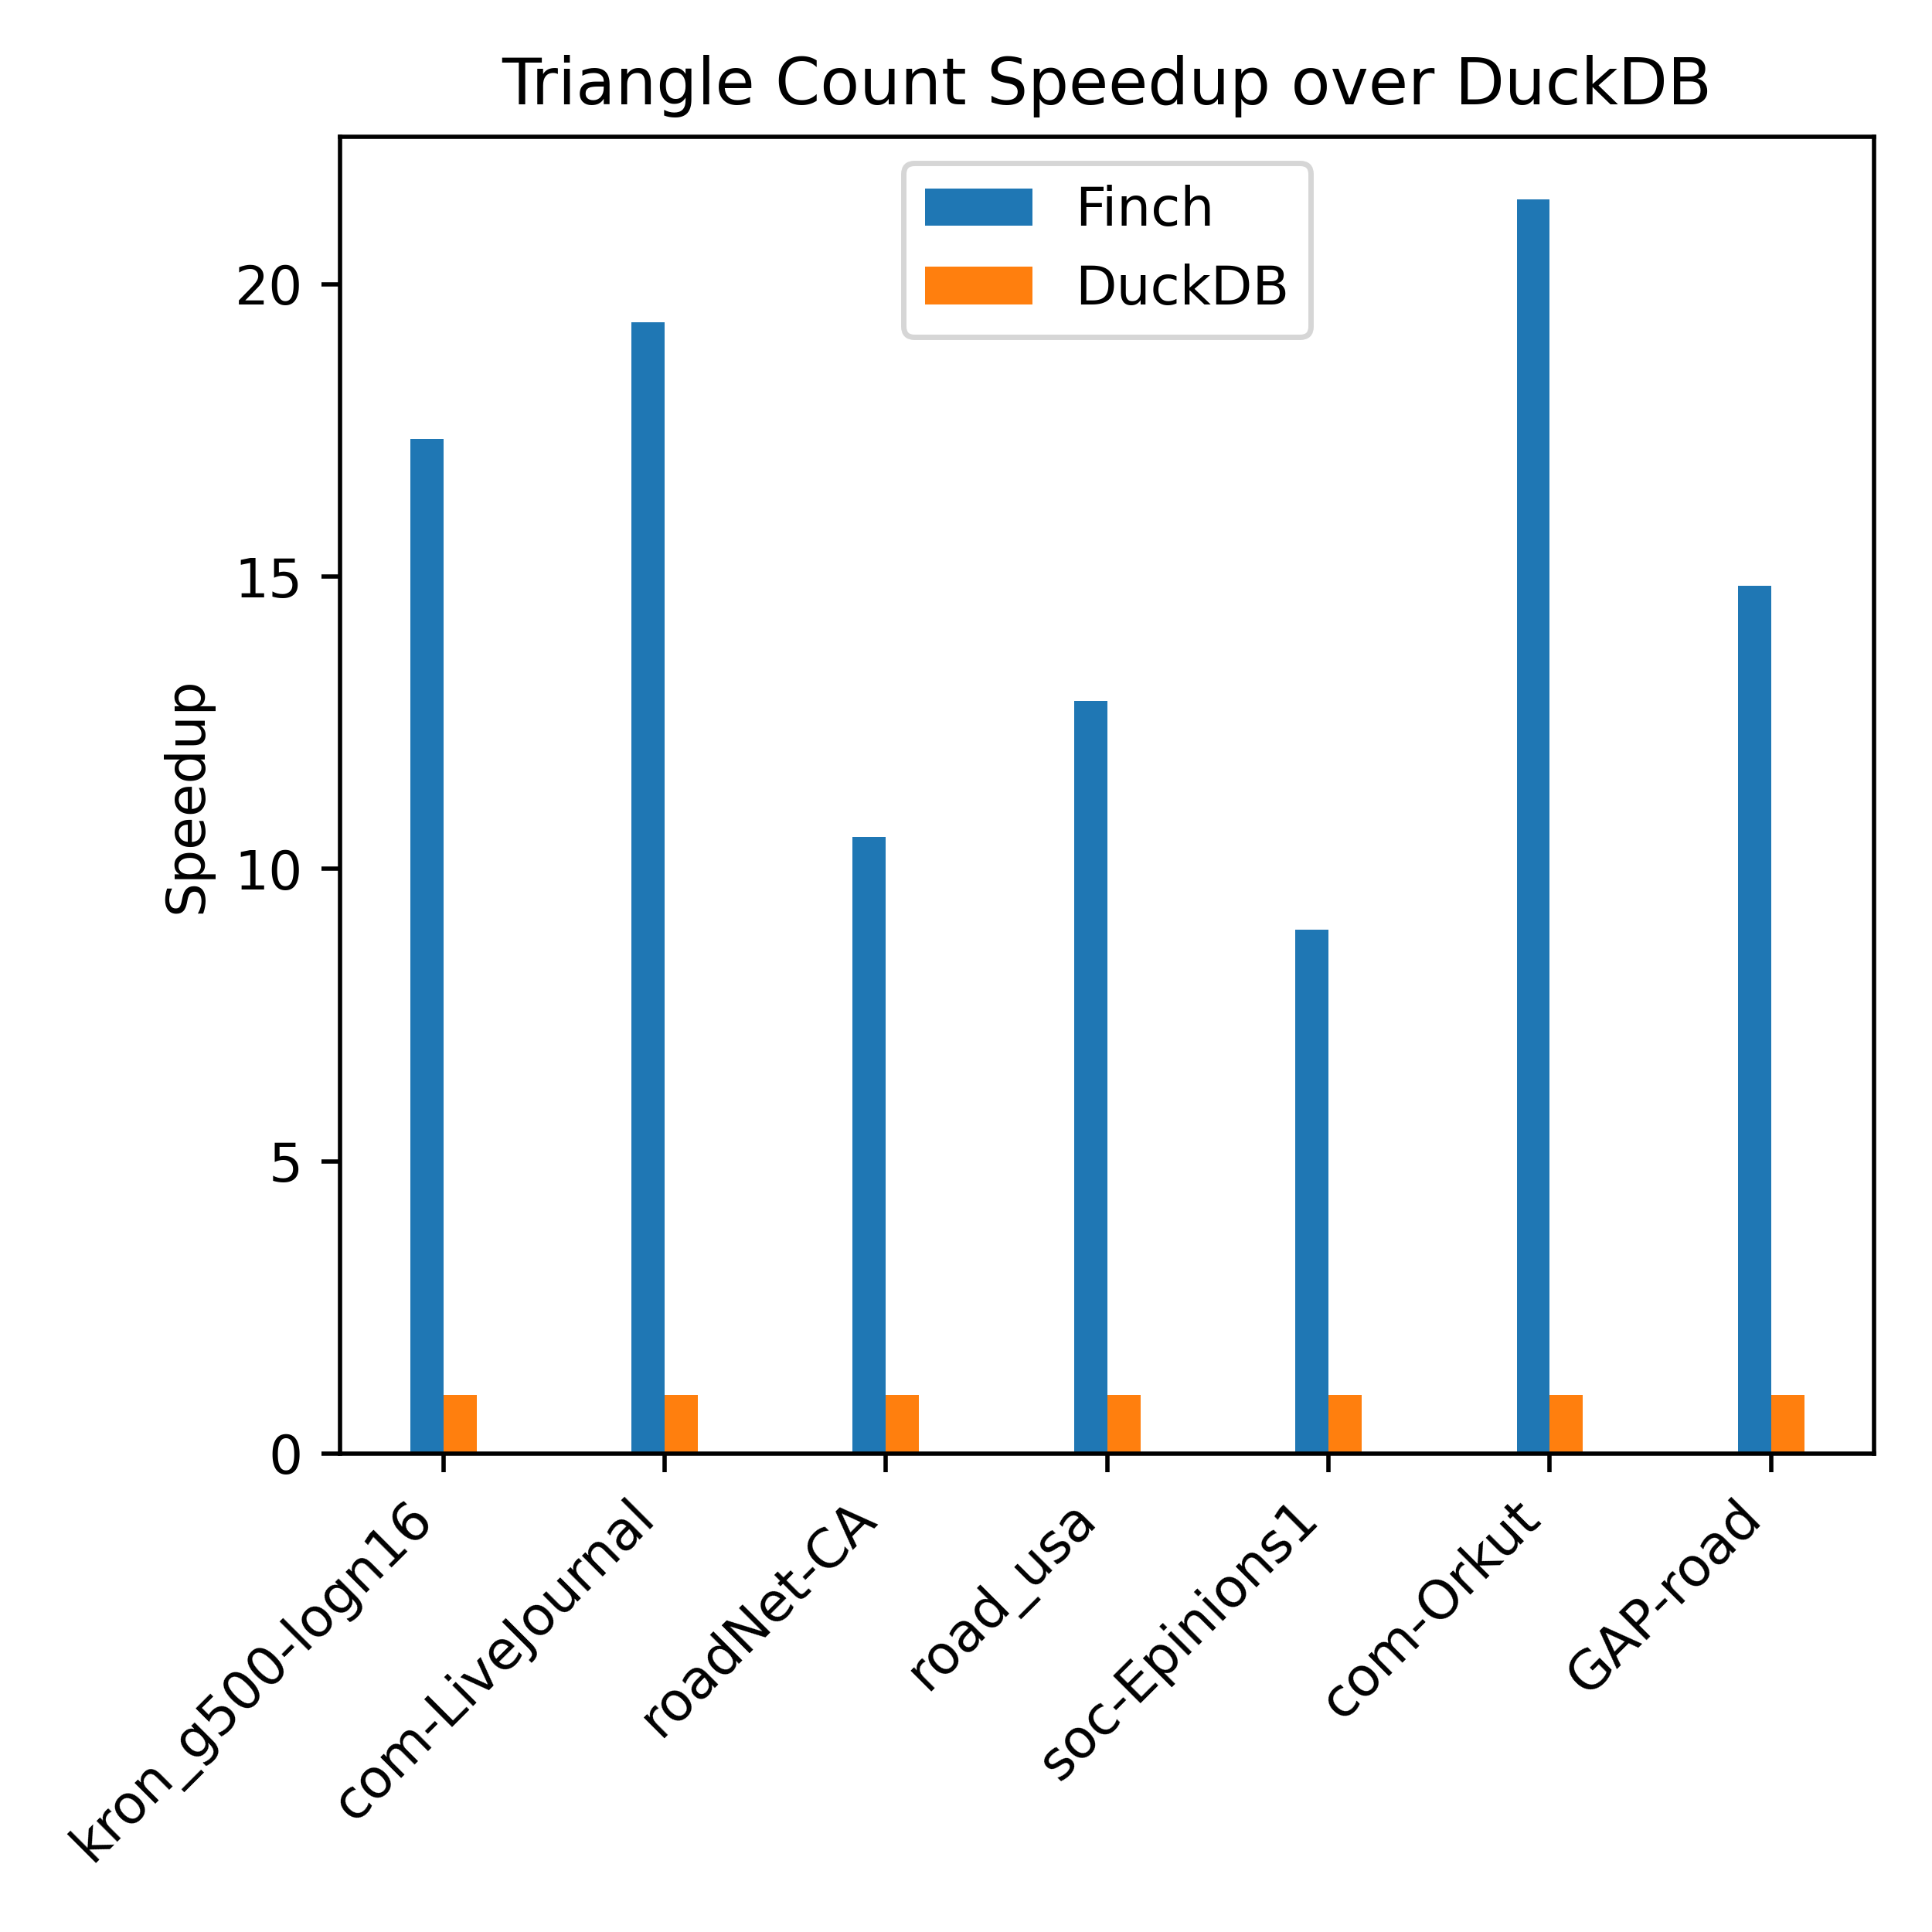
\includegraphics[width=140pt, height=135pt]{figures/triangle_count_speedup_over_duckdb.png} &
  \vspace{0pt} 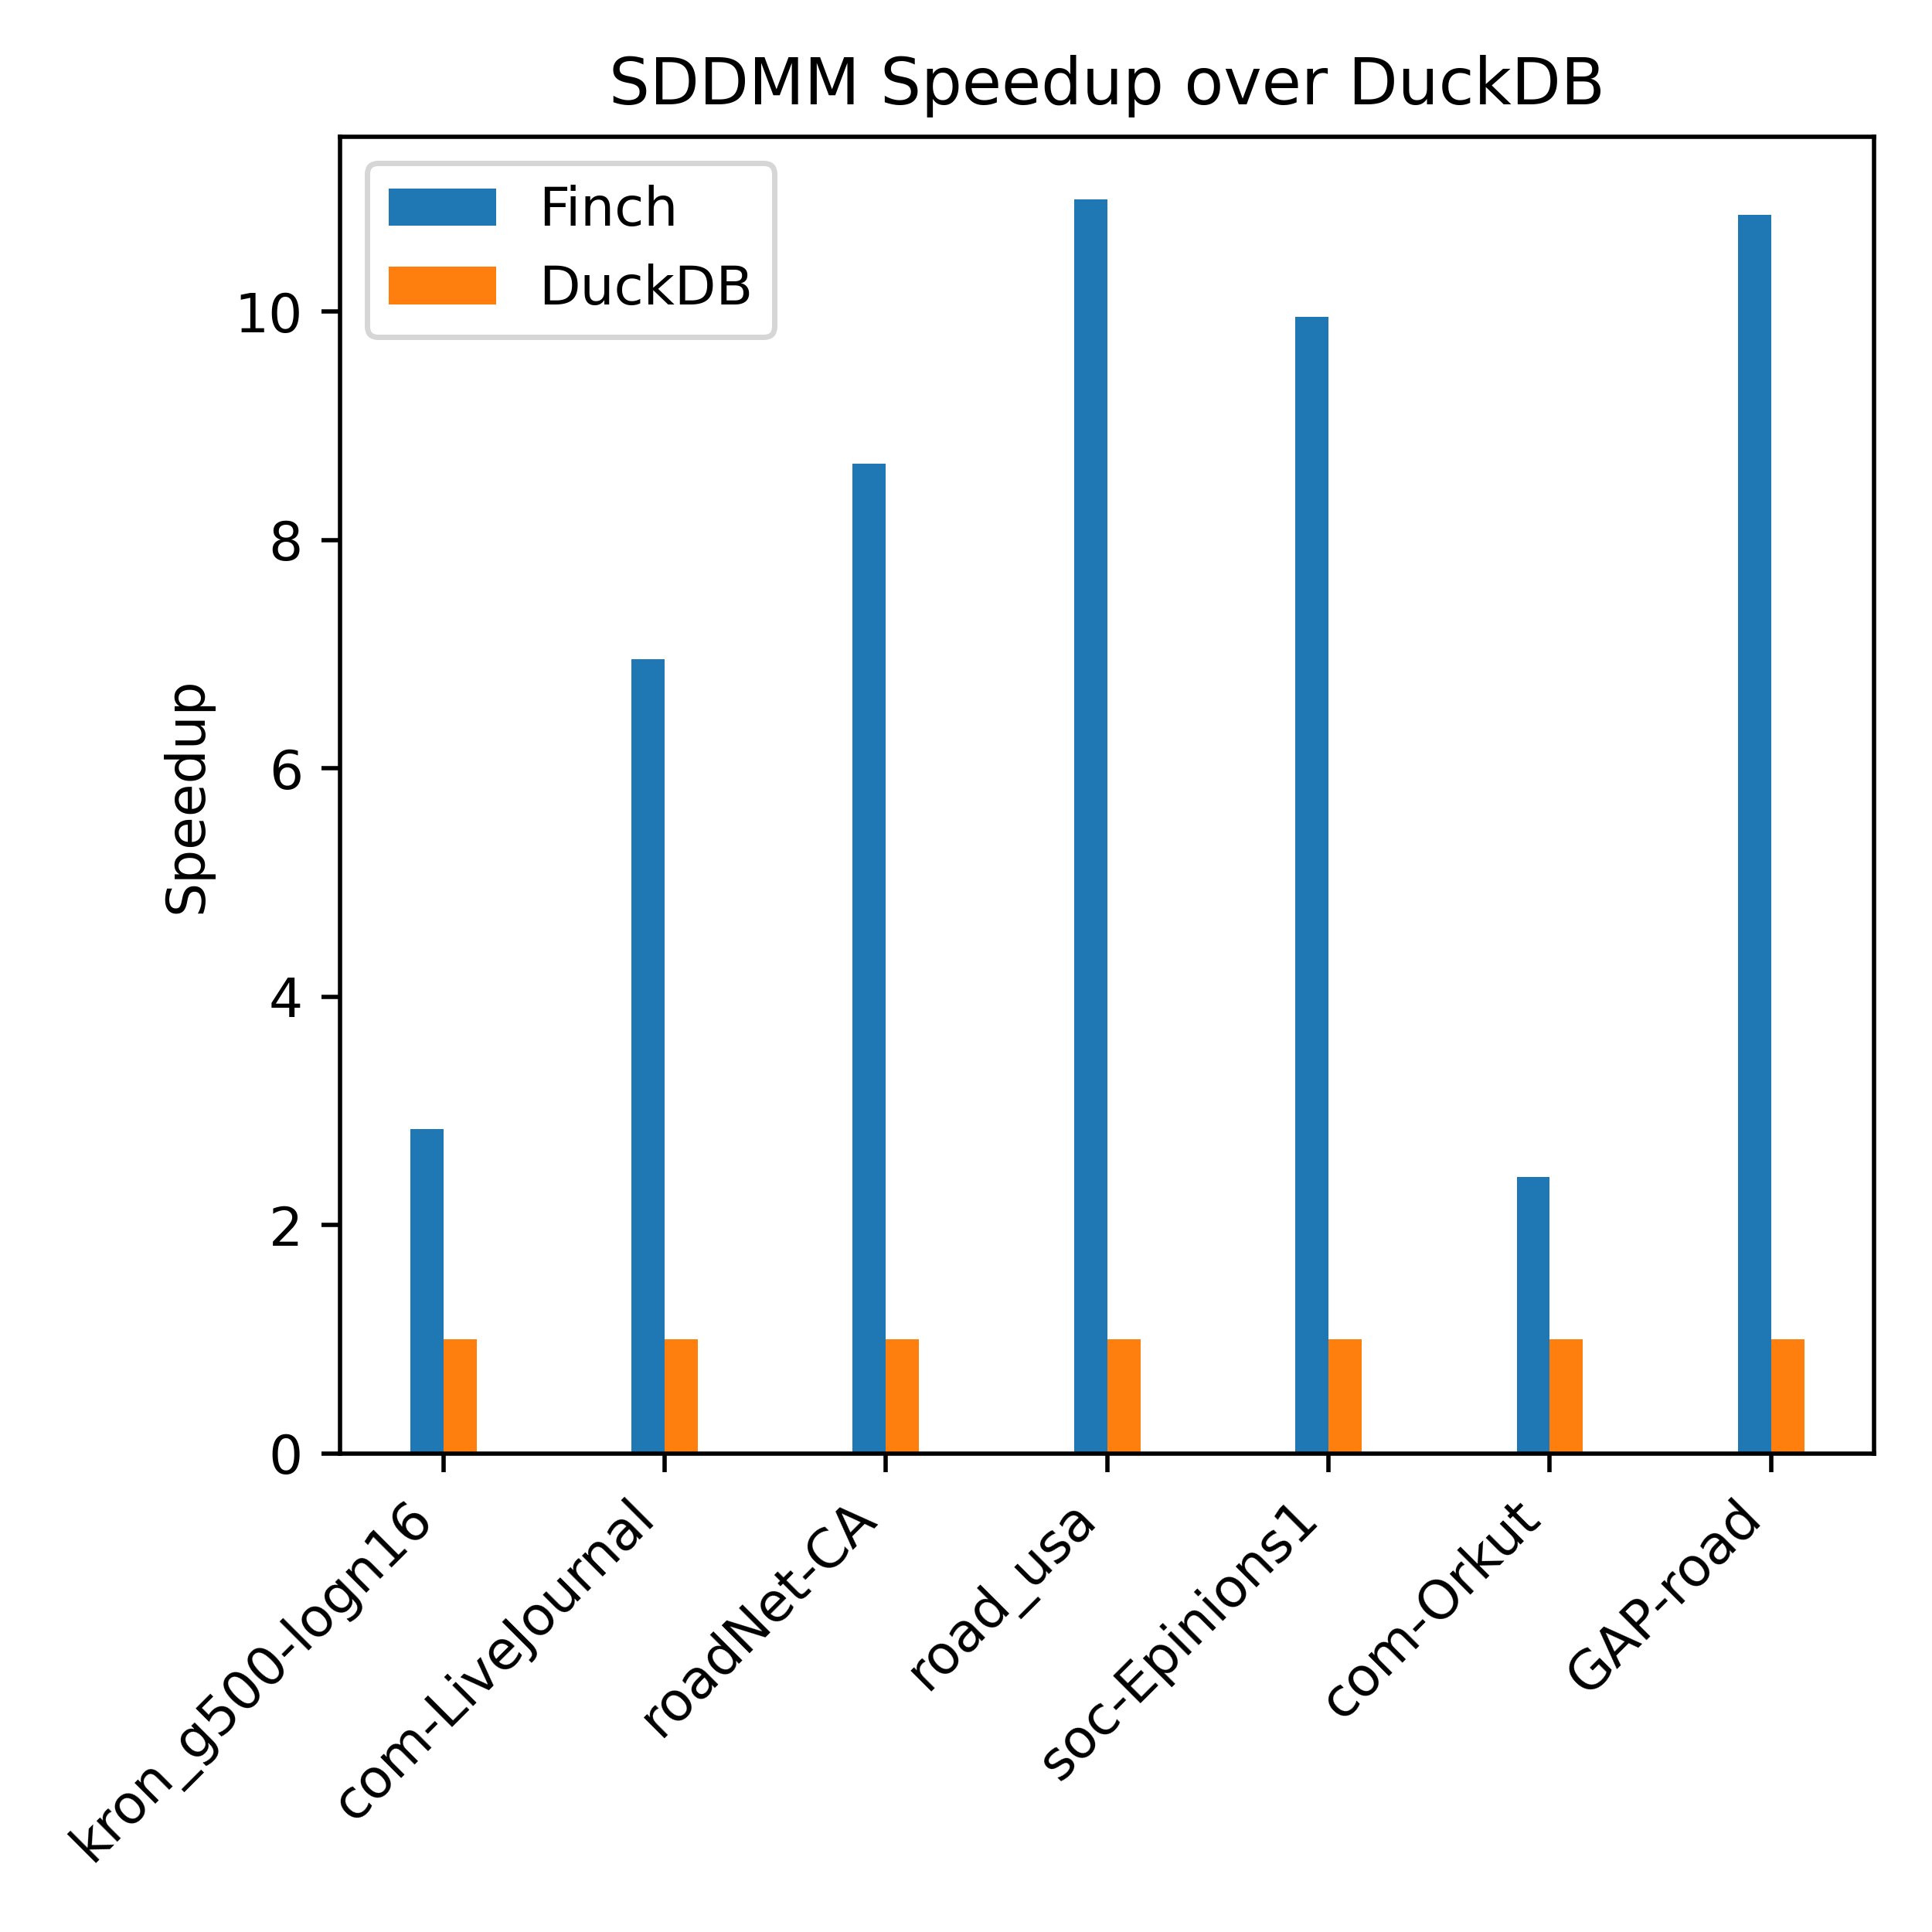
\includegraphics[width=140pt, height=135pt]{figures/sddmm_speedup_over_duckdb.png} &
  \vspace{0pt} 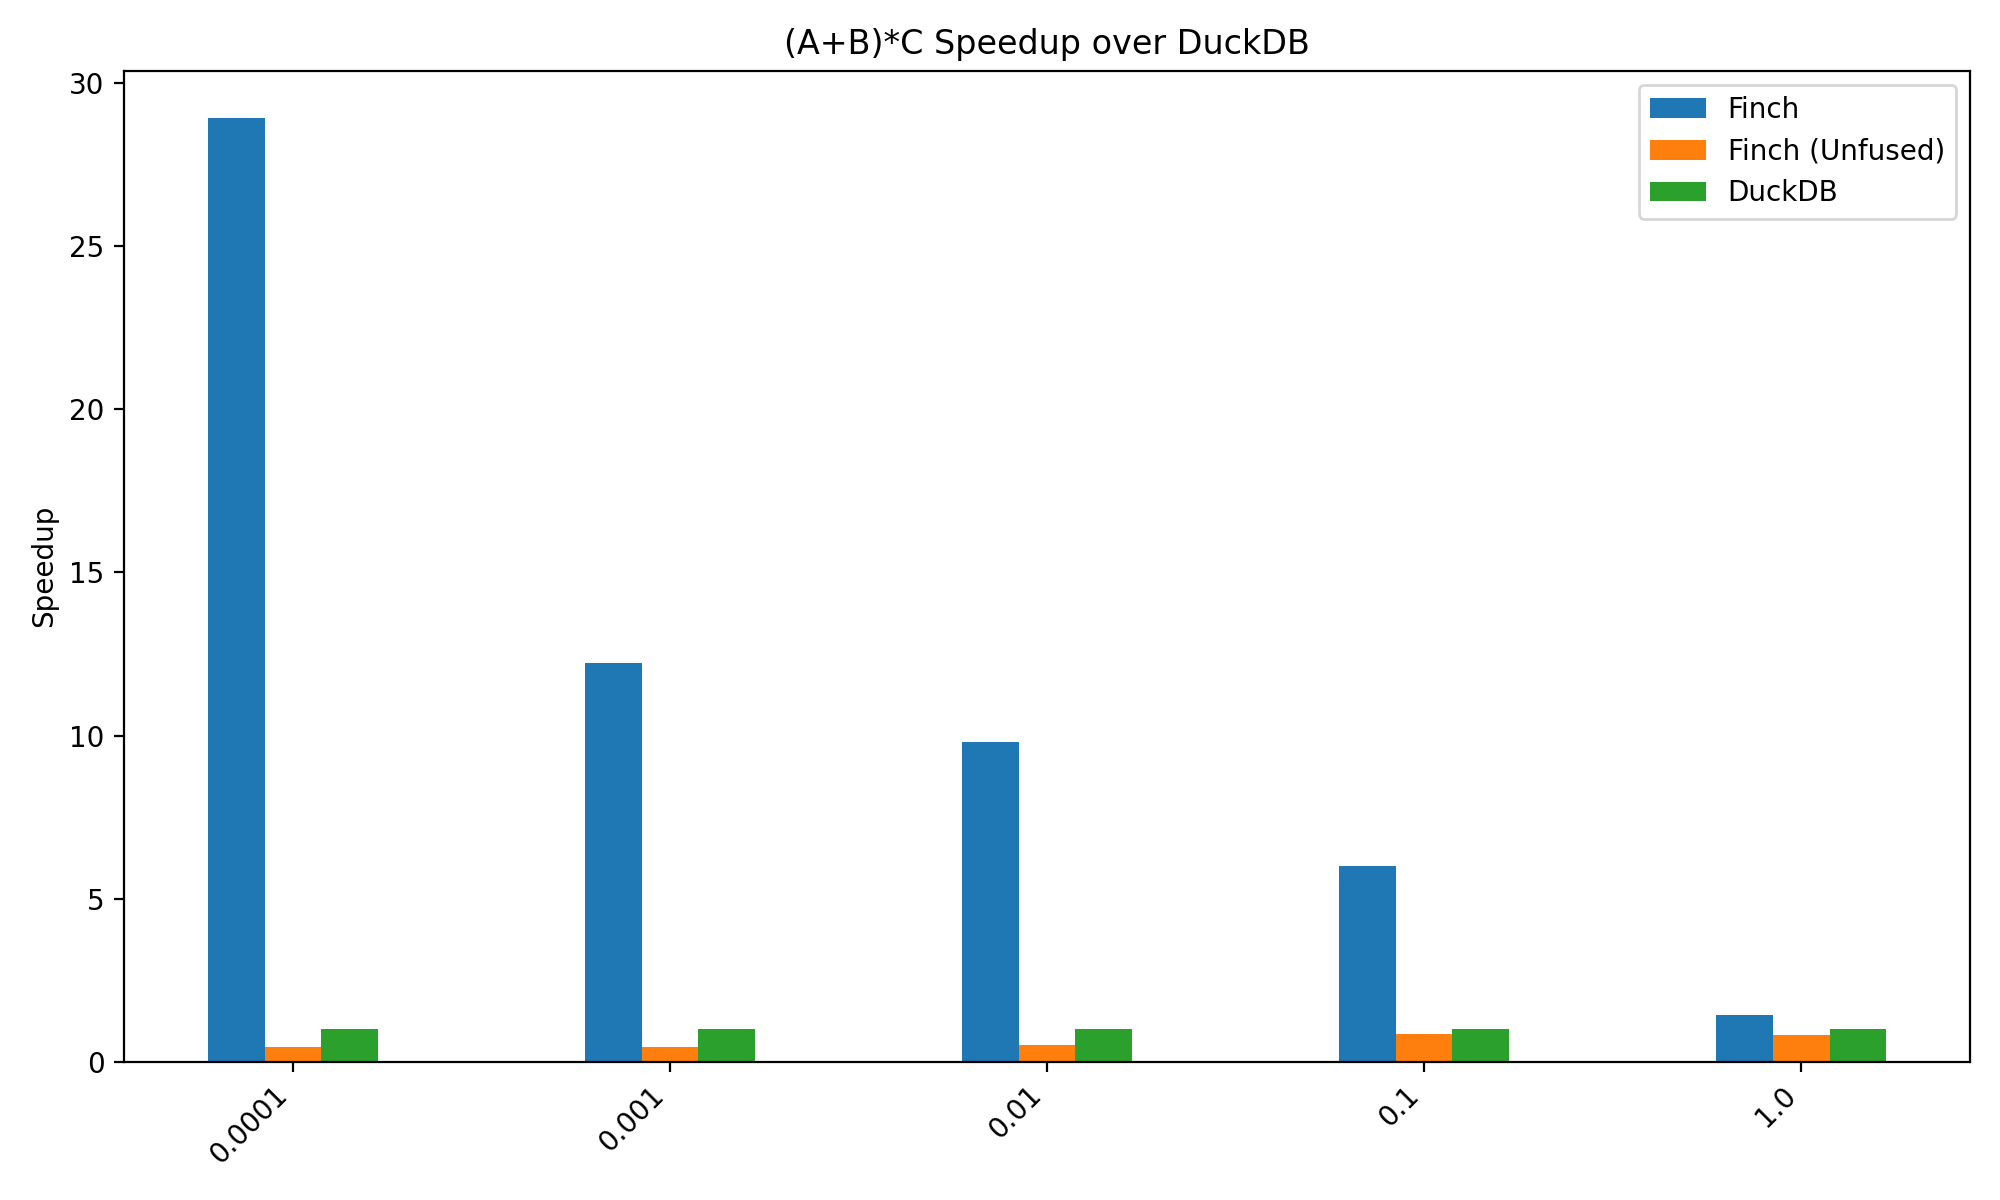
\includegraphics[width=140pt, height=123pt]{figures/elementwise_speedup_over_duckdb.png}
\end{tabular}
\vspace{-12pt}
\caption{Performance of Finch Logic for common kernels.} \label{fig:fusion}
\end{figure}




%matmul, mttkrp, repeated ttm, triangle counting, multiple pointwise,
%in-place.
%dot((v^t .* u), w)) vs. 
%(v^t .* dot(u, w))

\willow{Note: I may want to explain format inference somewhere in here, but I'll
have to get to it a little later, perhaps after the paper deadline}
\willow{Note: I think it would be cool to include something about how we support
numerically stable norms and argmin in this model}